\section{Deep Nueral Network}

\begin{table}[htpb]
    \centering
    \caption{Some short unfamiliar terminologies in Neural Network}
    {\footnotesize

}
    {\small
    \begin{tabular}{rp{28em}}
        \toprule
        Terminology & Brief definition \\
        \midrule
        \textbf{perceptron} & $f(\bm{x};\bm{\theta})=\mathbb{I}(\bm{w}^\mathsf{T}\bm{x}+b\geq 0)=H(\bm{w}^\mathsf{T}\bm{x}+b)$, where $H:\mathbb{R}\to\{0,1\}$ \\
        \textbf{vanishing gradient problem} & In the saturated regimes, the gradient of the output wrt the input will be close to zero, so any gradient signal from higher layers will not be able to propagate back to earlier layers. \\
        % \textbf{vanishing/exploding gradient problem} &  The gradient of a very deep models tends to become very small or large.\\
        \textbf{spectral radius} & of a matrix, which is the maximum of the absolute values of the eigenvalues. \\
        \textbf{gradient clipping} & $\bm{g}'=\bm{g}\min(1,\frac{c}{\|\bm{g}\|})$, keep the direction but the norm can never exceed $c$. \\
        \textbf{Xavier/Glorot initialization} & $w_{ij}\sim\mathcal{N}(0,2/(n_\text{in}+n_\text{out}))$,
        where $n_\text{in}$ and $n_\text{out}$ are the number of incoming and outgoing connections, respectively. 
        {\color{blue}(linear, tanh, logistic, and softmax)}\\
        \textbf{LeCun initialization} & $w_{ij}\sim\mathcal{N}(0,1/n_\text{in})$ {\color{blue}SELU}\\
        \textbf{He initialization} & $w_{ij}\sim\mathcal{N}(0,2/n_\text{in})$ 
        {\color{blue}ReLU, and its variants} \\
        \textbf{Uniform initialization} & $w_{ij}\sim\mathrm{Unif}(-a,a)$, where $a=\sqrt{6/(n_\text{in}+n_\text{out})}$ \\
        \textbf{layer-sequential unit-variance} & LSUV initialization, 
        (i) initialize $\mathbf{W}$ of all full\&convolutional layers by \textit{orthonormal matrices};
        (ii) for each layer $l$, rescale $\mathbf{W}_l\leftarrow\mathbf{W}_l/\sqrt{v_l}$, $v_l$ is the activations across \textit{a minibatch}.\\
        \textbf{weight decay} & equivalent to Gaussian prior or $\ell_2$ regularization, used in neural network literature \\
        \textbf{sparse DNNs} & generated by $\ell_1$ regularization or ARD for model compression, saving memory and time \\
        \textbf{Monte Carlo dropout} & $p(\bm{y}|\bm{x},\mathcal{D})\approx\frac{1}{S}\sum_{s=1}^S p(\bm{y}|\bm{x},\hat{\mathbf{W}}\bm{\epsilon}^s+\hat{\bm{b}})$, equivalent to ensemble of slightly different networks \\
        \textbf{Bayesian neural network} & $p(\bm{y}|\bm{x},\mathcal{D})=\int{p(\bm{y}|\bm{x},\bm{\theta})p(\bm{\theta}|\mathcal{D})}d\bm{\theta}$, an infinite ensemble of differently weighted neural networks \\
        \bottomrule
    \end{tabular}}
    \label{tab:newtermnetwork}
\end{table}




\subsection{Neural Network for Tabular Data}

The relationship between \textbf{basis function expansion} and \textbf{neural network}:
the former transfers original feature by a fixed manner or manually, 
which is not involved with parameters:
$\bm{x} \leftarrow \phi(\bm{x})$, and only updates $\bm{\theta}=(\mathbf{W},\bm{b})$; 
the latter learns the feature transformation by parameterizing it and updating 
over model fitting: $\bm{x} \leftarrow \phi(\bm{x};\bm{\theta}_2)$, 
and updates $\bm{\theta}=((\mathbf{W},\bm{b}),\bm{\theta}_2)$

\textbf{Multilayer perceptron (MLP)} or feedforward neural network (FFNN), whose DAG is a chain. The original version of MLP is to simulate logical functions by \text{heaviside step function}, $H$, and manually set weights and biases since $H$ is undifferentiable. 
The differentiable MLP replaces $H$ with a differentiable \textbf{activation function}
$\varphi:\mathbb{R}\to\mathbb{R}$
\begin{gather}
    f(\bm{x};\bm{\theta})
    = f_L(f_{L-1}(\cdots f_1(\bm{x};\bm{\theta}_1)\cdots;\bm{\theta}_{L-1});\bm{\theta}_L)\\
    \bm{z}_l=f_l(\bm{z}_{l-1};\bm{\theta}_l)=\varphi_l(\mathbf{W}_l\bm{z}_{l-1}+\bm{b}_l)
\end{gather}


MLP for \textbf{heteroskedastic regression}:\unsure{
Recall the \textbf{homoscedastic} and \textbf{heteroskedastic} regression,
which is first represented in 2.6.3 Regression and not included in notes before.
\textbf{homoscedastic regression} assumes that the variance is fixed, and is independent of the input, and, furthermore, \textbf{linear regression} assume the mean is a linear function of the input,
$p(y|\bm{x};\bm{\theta})=\mathcal{N}(y|\bm{w}^\mathsf{T}\bm{x}+b,\sigma^2)$.
While, \textbf{d heteroskedastic regression} assumes that the variance also depend on the input,
$p(y|\bm{x};\bm{\theta})=\mathcal{N}(y|\mu(\bm{x};\bm{\theta}_\mu),\sigma_+(\bm{x};\bm{\theta}_\Sigma))$
} 
use a shared backbone to extract nonlinear representation of original input $\bm{x}$,
and map it into mean and variance of modeling by two heads with specific parameters%, such as \unsure{
% One example is variational autoencoder.
% }
\begin{gather}
    p(y|\bm{x};\bm{\theta})
    = \mathcal{N}\left(
        y|\bm{w}_\mu^\mathsf{T}\bm{f}(\bm{x};\bm{w}_\text{shared}),
        \sigma_+(\bm{w}_\sigma^\mathsf{T}\bm{f}(\bm{x};\bm{w}_\text{shared})
    \right)\label{eq:heteroreg}
\end{gather}

Single layer MLP is a \textbf{universal function approximator}, 
with the capacity of modeling any suitably smooth function 
if given enough hidden units (wide but shallow architecture),
because each hidden unit can specify a half plane 
and a sufficient large combination of them can ``carve up'' any region of space.
However, the deep networks work better than shallow ones with the same units, 
since the features can be composed or hierarchical after getting through the earlier layers.

\textbf{Automatic differentiation}: 
repetitively applying the \textbf{chain rule} of calculus 
to a series of functions stacked as arbitrary DAGs (e.g. the simplest one is the form of sequence.),
i.e. $\bm{o}=\bm{f}(\bm{x})$, where $\bm{x}\in\mathbb{R}^n$, $\bm{o}\in\mathbb{R}^m$, 
and $\bm{f}=\bm{f}_4\circ\bm{f}_3\circ\bm{f}_2\circ\bm{f}_1:\mathbb{R}^n\to\mathbb{R}^m$ is a composition of functions: 
$\bm{f}_1:\mathbb{R}^n\to\mathbb{R}^{m_1}$, $\bm{f}_2:\mathbb{R}^{m_1}\to\mathbb{R}^{m_2}$, 
$\bm{f}_3:\mathbb{R}^{m_2}\to\mathbb{R}^{m_3}$, and $\bm{f}_4:\mathbb{R}^{m_3}\to\mathbb{R}^{m}$,
and denote the intermediate values as $\bm{x}_2=\bm{f}_1(\bm{x})$, $\bm{x}_3=\bm{f}_2(\bm{x}_2)$,
$\bm{x}_4=\bm{f}_3(\bm{x}_3)$, and $\bm{o}=\bm{f}_4(\bm{x}_4)$, then\unsure{
Recall the transformation of multiple r.v.s. 
The Jacobian matrix represent the local distortion relationship between two variables' space.
Similarly, for a composition of functions, $\mathcal{L}$, 
if we would like to compute the gradient wrt parameters $\bm{\theta}_k$ of any intermediate function $\bm{f}_k$ for the final output ($\mathcal{L}$),
the intractable method is to find the chain of deformation from $\bm{f}_k$ to the final output
and the differentiation of $\mathcal{L}$ wrt $\bm{\theta}_k$ is only required on $\bm{f}_k$ itself.
The final gradient spring out by the production between $\mathbf{J}$ and local gradient $\frac{\partial\bm{f}_k}{\partial\bm{\theta}_k}$.
}
\begin{align}
    \mathbf{J}_{\bm{f}}(\bm{x})
    = \frac{\partial\bm{f}(\bm{x})}{\partial\bm{x}} 
    =&~ \frac{\partial\bm{o}}{\partial\bm{x}_4}
       \frac{\partial\bm{x}_4}{\partial\bm{x}_3}
       \frac{\partial\bm{x}_3}{\partial\bm{x}_2}
       \frac{\partial\bm{x}_2}{\partial\bm{x}} \\
    =&~ \frac{\partial\bm{f}_4(\bm{x}_4)}{\partial\bm{x}_4}
       \frac{\partial\bm{f}_3(\bm{x}_3)}{\partial\bm{x}_3}
       \frac{\partial\bm{f}_2(\bm{x}_2)}{\partial\bm{x}_2}
       \frac{\partial\bm{f}_1(\bm{x})}{\partial\bm{x}} \\
    =&~ \underbrace{\mathbf{J}_{\bm{f}_4}(\bm{x}_4)}_{m \times m_3}
        \underbrace{\mathbf{J}_{\bm{f}_3}(\bm{x}_3)}_{m_3 \times m_2}
        \underbrace{\mathbf{J}_{\bm{f}_2}(\bm{x}_3)}_{m_2 \times m_1}
        \underbrace{\mathbf{J}_{\bm{f}_1}(\bm{x})}_{m_1 \times n},
\end{align}
We can see that it will be more efficient to compute $\mathbf{J}_{\bm{f}}(\bm{x})$
from left to right if $m<n$, called \textbf{reverse mode differentiation}, 
by \textbf{Vector-Jacobian Product} (VJP).
\unsure{
However, the intermediate values, $\bm{x}_{2:4}$ and $\bm{o}$, 
should still be computed by forward mode and based on the parameters of the last updated.
(Forward pass before back propagation)}

\begin{example}
    \textbf{Automatic differentiation for MLP}
    
    Considering an MLP for regression with one hidden layer and squared loss
    \begin{gather}
        \mathcal{L}((\bm{x},\bm{y}),\bm{\theta}) 
        = \frac{1}{2}\|\bm{y}-\mathbf{W}_2\phi(\mathbf{W}_1\bm{x})\|_2^2
    \end{gather}
    Denote that
    \begin{align}
        \mathcal{L} =&~ \bm{f}_4\circ\bm{f}_3\circ\bm{f}_2\circ\bm{f}_1 \\
        \bm{x}_2 =&~ \bm{f}_1(\bm{x},\bm{\theta}_1) = \mathbf{W}_1\bm{x} \\
        \bm{x}_3 =&~ \bm{f}_2(\bm{x}_2,\varnothing) = \varphi(\bm{x}_2) \\
        \bm{x}_4 =&~ \bm{f}_3(\bm{x}_3,\bm{\theta}_3) = \mathbf{W}_2\bm{x}_3 \\
        \mathcal{L} =&~ \bm{f}_4(\bm{x}_4,\bm{y}) = \frac{1}{2}\|\bm{x}_4-\bm{y}\|^2
    \end{align}
    Then
    \begin{align}
        \nabla_{\bm{\theta}_3}\mathcal{L} 
        =&~ \mathbf{J}_{\bm{f}_4}(\bm{x}_4)
            \nabla_{\bm{\theta}_3}\bm{f}_3\\
        \nabla_{\bm{\theta}_2}\mathcal{L}
        =&~ \mathbf{J}_{\bm{f}_4}(\bm{x}_4)
            \mathbf{J}_{\bm{f}_3}(\bm{x}_3)
            \nabla_{\bm{\theta}_2}\bm{f}_2\\
        \nabla_{\bm{\theta}_1}\mathcal{L}
        =&~ \mathbf{J}_{\bm{f}_4}(\bm{x}_4)
            \mathbf{J}_{\bm{f}_3}(\bm{x}_3)
            \mathbf{J}_{\bm{f}_2}(\bm{x}_2)
            \nabla_{\bm{\theta}_1}\bm{f}_1
    \end{align}
\end{example}

Jacobian Matrix for several common layers: recall the form of \textbf{Jacobian Matrix}: for a layer $\bm{f}:\mathbb{R}^n\to\mathbb{R}^m$, 
its Jacobian matrix is defined by 
\begin{gather}
    \mathbf{J}_{\bm{f}}(\bm{x})
    = \left[\frac{\partial f_i}{\partial x_j}\right]_{m\times n}
    = \left[\begin{array}{c}
        \nabla f_1(\bm{x})^\mathsf{T} \\
        \vdots \\
        \nabla f_m(\bm{x})^\mathsf{T}
    \end{array}\right]
    = \left[\frac{\partial}{\partial x_1}\bm{f},\cdots,\frac{\partial}{\partial x_n}\bm{f}\right]
    \in \mathbb{R}^{m\times n}
\end{gather}
\begin{enumerate}[{(1)}]
    \item Cross entropy layer: $\mathbb{R}^C\to\mathbb{R}$
    \unsure{NOTE: Like many other activation functions, softmax has no parameter.}
    \unsure{it is time consuming because the requirement of normalization across dimension, unavailable for paralleling.}
    \begin{align}
        z 
        =&~ f(\bm{x}) = \mathrm{CEWithLogits}(\bm{y},\bm{x}) \\
        =&~ -\sum_c y_c\log\mathrm{softmax}(\bm{x})_c = \sum_c y_c\log p_c \\
        \mathbf{J} 
        =&~ \frac{\partial z}{\partial \bm{x}}=(\bm{p}-\bm{y})^\mathsf{T}\in\mathbb{R}^{1\times{C}} 
    \end{align}
    \item Elementwise nonlinearity: $\mathbb{R}^n\to\mathbb{R}^n$
    \begin{align}
        \bm{z}
        =&~ \varphi(\bm{x}) = [\varphi(x_i)] \\
        \mathbf{J}
        =&~ \mathrm{diag}{(\varphi'(x_1),\cdots,\varphi'(x_n))} \\
        (=&~ \mathrm{diag}{(\mathbb{I}(x_1>0),\cdots,\mathbb{I}(x_n>0))}~\text{if}~\varphi=\mathrm{ReLU})
    \end{align}
    \item Linear layer: $\mathbb{R}^n\to\mathbb{R}^m$ (by a $m\times n$ matrix $\mathbf{W}=[w_{ij}]$)
    \begin{align}
        \bm{z}
        =&~ \bm{f}(\bm{x},\mathbf{W}) = \mathbf{W}\bm{x} \\
        \mathbf{J}
        =&~ \mathbf{W} 
    \end{align}
    The gradient of $\bm{f}$ wrt $\mathbf{W}$ is\unsure{
    Recall the gradient of $f(\mathbf{X}):\mathbb{R}^{m\times n}\to \mathbb{R}$ is $\frac{\partial f}{\partial \mathbf{X}}=\left[\frac{\partial f}{\partial X_{ij}}\right]\in\mathbb{R}^{m\times n}$
    } 
    \begin{align}
        \nabla_\mathbf{W}\bm{f}
        =&~ \left[\frac{\partial\bm{z}}{\partial w_{ij}}\right]\in\mathbb{R}^{m\times(m\times n)} \\
        \text{where}~\frac{\partial\bm{z}}{\partial w_{ij}}
        =&~ [0,\cdots,0,x_j,0,\cdots,0]^\mathsf{T} \\
        \Rightarrow\bm{u}^\mathsf{T}\frac{\partial\bm{z}}{\partial \mathbf{W}}
        =&~ \bm{ux}^\mathsf{T}\in\mathbb{R}^{m \times n}
    \end{align}
\end{enumerate}

\begin{example}
    \textbf{Automatic differentiation for General Complex Structures}

    The differentiation wrt data or parameters for other complex structure of data flow can be 
    implemented by \textbf{computation graph}:
    \begin{gather}
        \frac{\partial \bm{o}}{\partial \bm{x}_j} 
        = \sum_{k\in\mathrm{Children}(j)}
        \frac{\partial\bm{o}}{\partial\bm{x}_k}\frac{\partial\bm{x}_k}{\partial\bm{x}_j}
    \end{gather}
    Figure \ref{fig:compgraph} shows an example of computation graph.
\end{example}

\begin{figure}[htpb]
    \centering
    \begin{tikzpicture}[
    roundnode/.style={circle, draw=violet!60, fill=violet!5, minimum size=7mm},
    ->,>=stealth',auto,node distance=3.5em,thick,show background rectangle]
    \tikzstyle{every node}=[font=\small,scale=0.9]
      \node[]
      (anchor0)
      {};
      
      \node[above = of anchor0]
      (input1)
      {\color{teal}$\bm{x}_1$};
      
      \node[below = of anchor0]
      (input2)
      {\color{teal}$\bm{x}_2$};
      
      \node[roundnode, right = of input1]
      (func3)
      {$\bm{f}_3$};

      \node[right = of anchor0]
      (anchor1)
      {};
      
      \node[roundnode, right = of input2]
      (func4)
      {$\bm{f}_4$};
      
      \node[roundnode, right = of anchor1]
      (func5)
      {$\bm{f}_5$};

      \node[roundnode, right = of func5]
      (func6)
      {$\bm{f}_6$};
      
      \node[roundnode, right = of func6]
      (func7)
      {$\bm{f}_7$};

      \node[right = of func7]
      (x7)
      {$\bm{x}_7={\color{purple}\bm{o}}$};
      
      \draw[->] (input1)  --  (func3);
      \draw[->] (input1)  --  (func5);
      \draw[->] (input2)  --  (func4);
      \draw[->] (func3)  --node{$\bm{x}_3$}  (func4);
      \draw[->] (func4)  --node{$\bm{x}_4$}  (func5);
      \draw[->] (func4)  --node{$\bm{x}_4$}  (func7);
      \draw[->] (func5)  --node{$\bm{x}_5$}  (func6);
      \draw[->] (func6)  --node{$\bm{x}_6$}  (func7);
      \draw[->] (func7)  --  (x7);
    \end{tikzpicture}
    \caption{Example for the computation graph of $f(\bm{x}_1,\bm{x}_2)=x_2e^{x_1}\sqrt{x_1+x_2e^{x_1}}$}
    {\footnotesize
    \begin{align*}
        x_3 &=~ f_3(x_1) = e^{x_1} \\
        x_4 &=~ f_4(x_2,x_3) = x_2x_3 \\
        x_5 &=~ f_5(x_1,x_4) = x_1 + x_4 \\
        x_6 &=~ f_6(x_5) = \sqrt{x_5} \\
        x_7 &=~ f_7(x_4,x_6) = x_4x_6
    \end{align*}
    }
    \label{fig:compgraph}
\end{figure}

\begin{figure}[htpb]
    \centering
    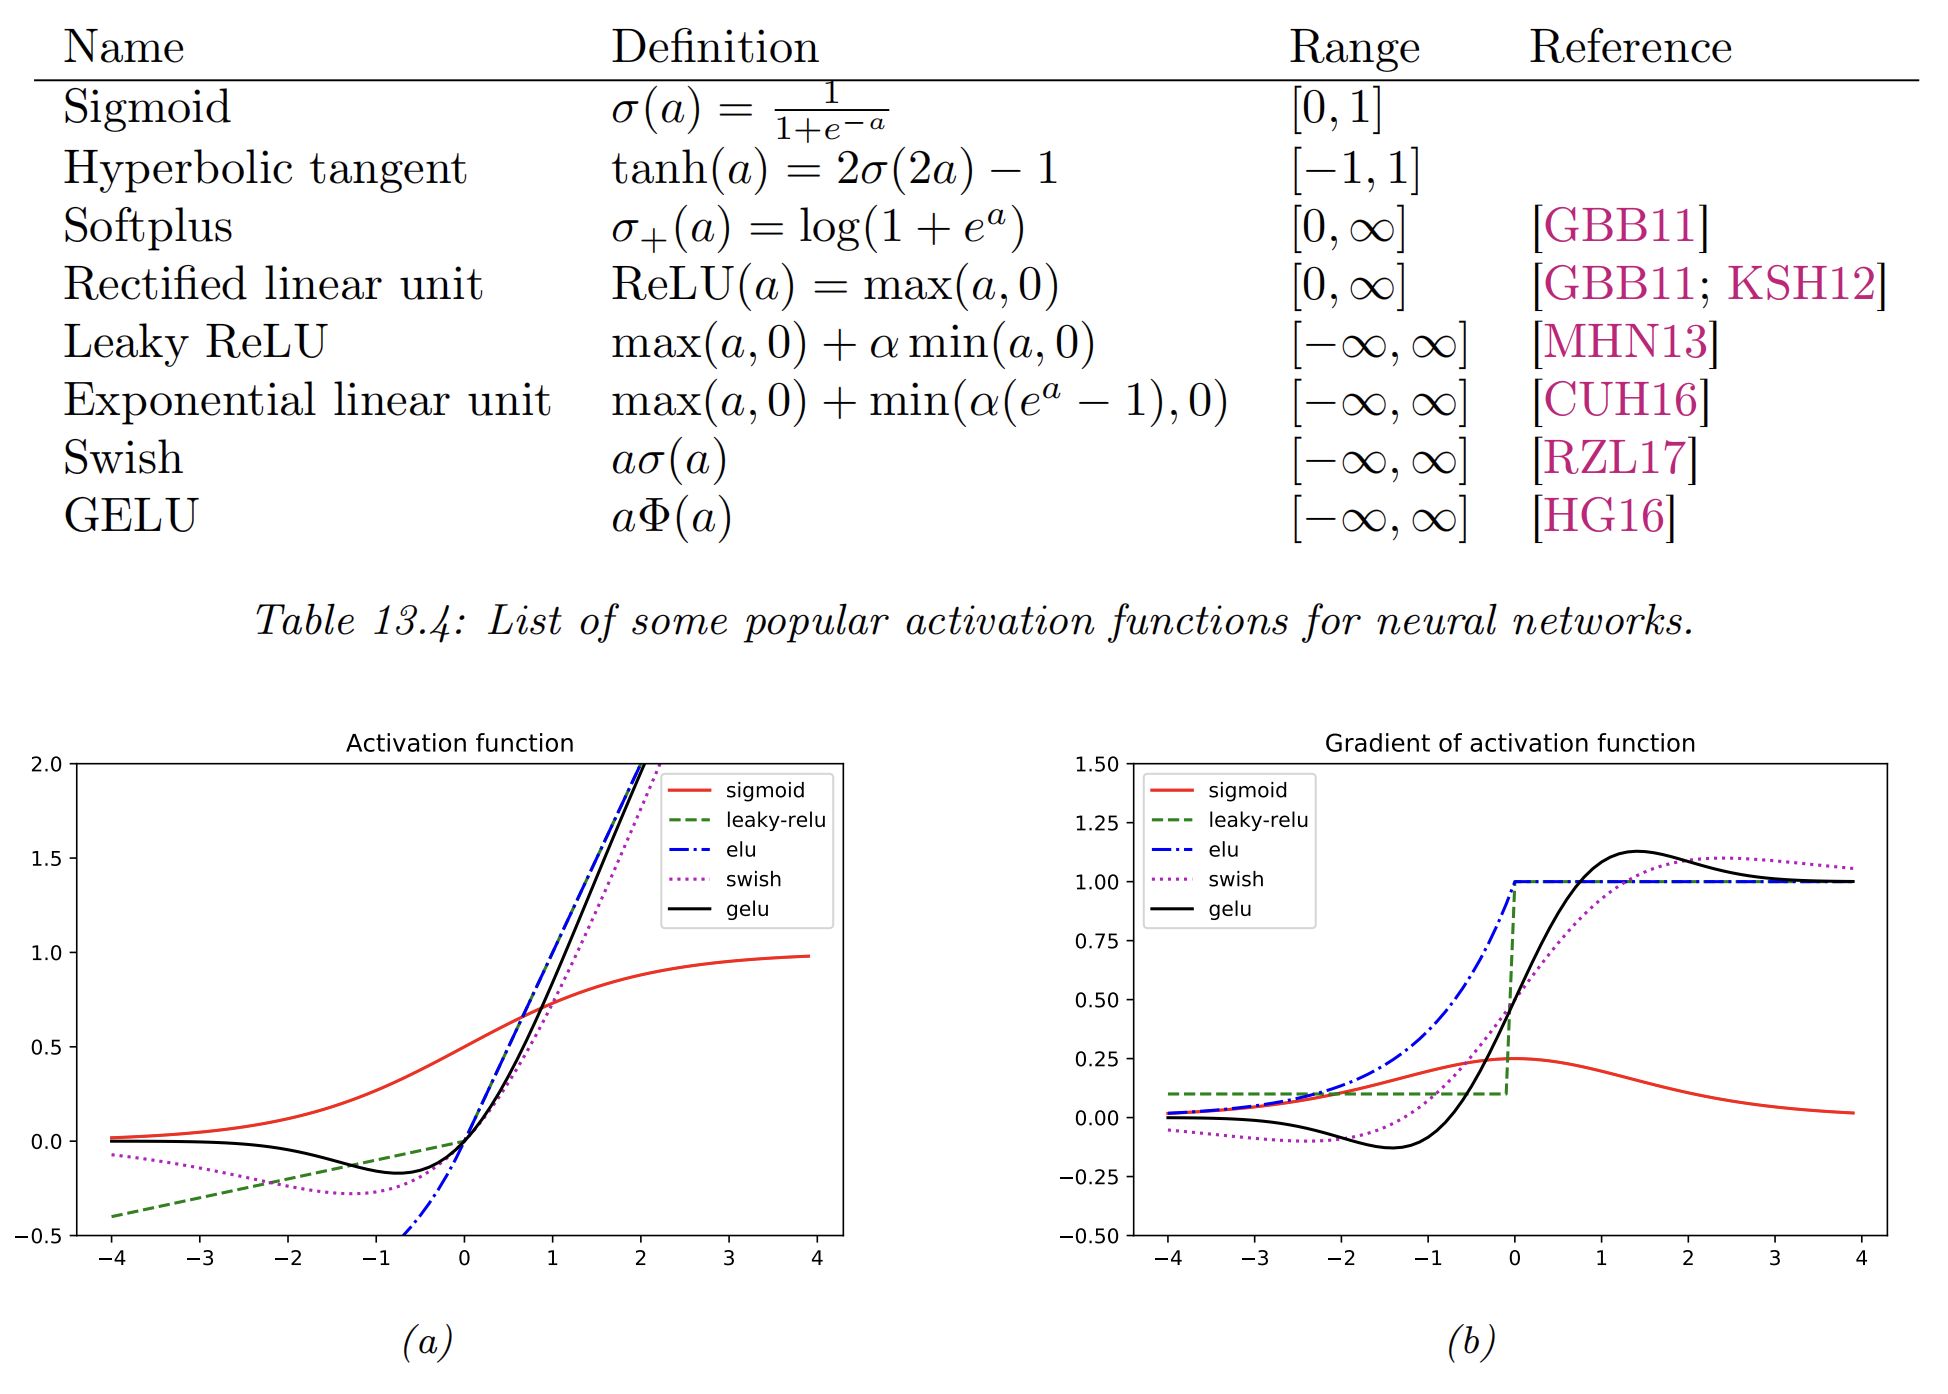
\includegraphics[width=0.75\textwidth]{figs/activationfunc.png}
    \caption{Some popular activation functions and their gradients}
    \label{fig:activationfunc}
\end{figure}

Strategies of solving vanishing gradient problems:
\begin{enumerate}[{(1)}]
    \item modify the activation function to be with proper gradient (e.g \textbf{non-saturating activation functions} in Figure \ref{fig:activationfunc});
    \item modify the architecture to addtively rather than multiplicatively update;
    \item modify the architecture to standardize the activations at each layers (e.g. residual connection in architecture explained below);
    \item carefully choose the initial values of the parameters 
    (e.g. for standard ReLU, the gradient will never escape from zero 
    if the initialized weights such that $\mathbf{W}\bm{x}$ is a large negative value, 
    called \textbf{dead ReLU}. 
    This problem is solved by Leaky ReLU that allows small gradient in the region of negatives.).
\end{enumerate}

\textbf{Residual connections}: 
the layer in a \textbf{residual block} only computes the residual term 
that needs to be added to the input $\bm{x}$ to generate the desired output, 
which does not introduce extra parameters but will be more easy to learn/train.\unsure{
NOTE: The residual connection addition is element-wise, and after an input gets through a residual block, its dimension will not be changed.
}
\begin{gather}
    (\bm{x}_{l+1}=)\Tilde{\bm{f}}_l(\bm{x_l};\bm{\theta}_l) = \bm{f}_l(\bm{x_l};\bm{\theta}_l)+\bm{x}_l\\
    \Rightarrow 
    \Tilde{\bm{f}}(\bm{x};\bm{\theta}_{1:L}) 
    = \Tilde{\bm{f}}_L(\cdots\Tilde{\bm{f}}_l(\bm{x}_l;\bm{\theta}_l)\cdots,\bm{\theta}_L) 
    = \bm{x}_l + \sum_{i=l}^{L}\bm{f}_i(\bm{x}_i;\bm{\theta}_i) \\
    \Rightarrow
    \frac{\partial\mathcal{L}}{\partial\bm{\theta}_l}
    = \frac{\partial\bm{x}_{l}}{\partial\bm{\theta}_l}
      \frac{\partial\mathcal{L}}{\partial\bm{x}_{L}}
      \frac{\partial\bm{x}_{L}}{\partial\bm{x}_{l}}
    = \frac{\partial\bm{x}_{l}}{\partial\bm{\theta}_l}
      \frac{\partial\mathcal{L}}{\partial\bm{x}_{L}}
      \underbrace{\left(
        1 + \sum_{i=l}^{L-1}\frac{\partial\bm{f}_i(\bm{x}_i;\bm{\theta}_i)}{\partial\bm{x}_l}
      \right)}_{\text{other terms}}
\end{gather}
which shows the gradient at layer $l$ can depend directly on the gradient at layer $L$ 
in a way that is independent of the depth of the network.\unsure{
But I am not very sure what is $\frac{\bm{x}_l}{\bm{\theta}_l}$. 
Is it equal to zero since $\bm{x}_l$ and $\bm{\theta}_l$ act as the inputs at the same time 
for a layers and have nothing to do with each other?}

\begin{figure}[htpb]
    \centering
    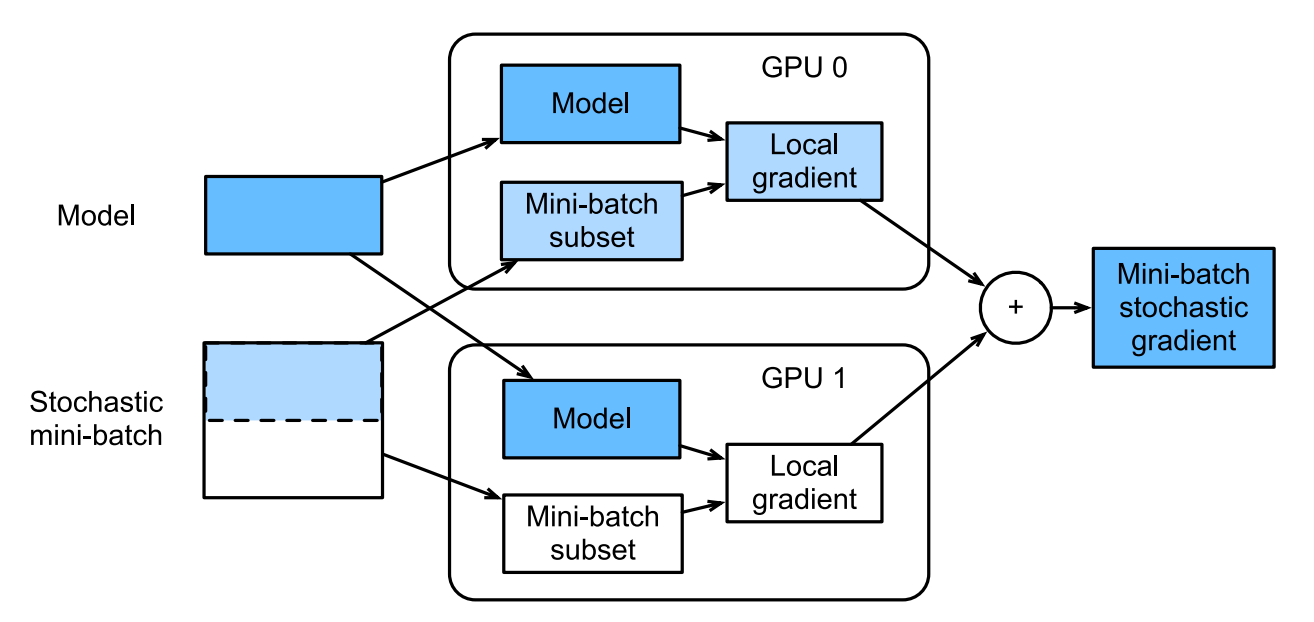
\includegraphics[width=0.75\textwidth]{figs/paralleltrain.png}
    \caption{Parallel training across multiple machines}
    \label{fig:paralleltrain}
    {\footnotesize 
    \textbf{synchronous training}: Each machine \textit{blocks} until receiving the centrally aggregated gradient $\bm{g}_t$, 
    $\Tilde{\bm{g}}_t^k\leftarrow\sum_{k=1}^K\bm{g}_t^k$, 
    and $\bm{\theta}_t^k\leftarrow\bm{\theta}_t^k-\eta_t\Tilde{\bm{g}}_t^k$.
    
    Otherwise, \textbf{asynchronous training}, no aggregation of $\bm{g}_t$ 
    but $\bm{\theta}_t^k\leftarrow\bm{\theta}_t^k-\eta_t\bm{g}_t^k$}
\end{figure}

Other kinds of feedforward networks:
\begin{enumerate}[{(1)}]
    \item 
    \textbf{Radial basis function (RBF) network}: 
    Given a set of $K$ \textit{centroids} or \textit{exemplars}, $\bm{\mu}_k\in\mathcal{X}$\unsure{
    compute the RBF similarity between data points and these outstanding exemplars.
    }
    \begin{gather}
        \phi(\bm{x}) 
        = \left[\mathcal{K}(\bm{x},\bm{\mu}_i)\right]:\mathbb{R}^D\to\mathbb{R}^{K}\\
        \mathcal{K}_\text{gauss}(\bm{x},\bm{c})
        \triangleq \exp\left(-\frac{1}{2\sigma^2}\|\bm{x}-\bm{c}\|_2^2\right) \\
        \begin{cases}
        p(y|\bm{x},\bm{\theta}) = \mathcal{N}(\bm{w}^\mathsf{T}\phi(\bm{x},\sigma^2)) & \text{for regression} \\
        p(y|\bm{x},\bm{\theta}) = \mathrm{Ber}(\sigma(\bm{w}^\mathsf{T}\phi(\bm{x}))) & \text{for classification}
        \end{cases}
    \end{gather}
    \item 
    \textbf{Mixture of linear experts}: a conditional mixture model that regresses multiple outputs that conditioned a certain source, called \textit{expert}\unsure{
    recall the mixture model of Gaussian distributions
    }
    % heteroskedastic regression like Equation (\ref{eq:heteroreg}) will give certain $x$ values two equally probable $y$ values, called \textbf{one-to-many functions}.
    \begin{align}
        p(\bm{y}|\bm{x}) =&~ \sum_{k=1}^K p(\bm{y}|\bm{x},z=k)p(z=k|\bm{x}) \\
        p(\bm{y}|\bm{x},z=k) =&~ \mathcal{N}(\bm{y}|f_{\mu,k}(\bm{x}),\mathrm{diag}(f_{\sigma,k}(\bm{x}))) \\
        p(z=k|\bm{x}) =&~ \mathrm{Cat}(z|\mathrm{softmax}(f_z(\bm{x})))
    \end{align}
\end{enumerate}



